\documentclass[a4paper,11pt]{article}
\input{/home/tof/Documents/Cozy/latex-include/preambule_lua.tex}
\newcommand{\showprof}{show them}  % comment this line if you don't want to see todo environment
\fancyhead[L]{TP système d'exploitation}
\newdate{madate}{10}{09}{2020}
\fancyhead[R]{Première - NSI} %\today
\fancyfoot[L]{~\\Christophe Viroulaud}
\fancyfoot[C]{\textbf{Page \thepage}}
\fancyfoot[R]{\includegraphics[width=2cm,align=t]{/home/tof/Documents/Cozy/latex-include/cc.png}}

\begin{document}
\begin{Form}
\section{Problématique}
L'interface graphique (matérialisée par \emph{le bureau}) est le principal mode d'interaction entre la machine et l'utilisateur. Il est ainsi aisé de créer un nouveau dossier dans l'espace disque, avec la souris. Mais ce système graphique n'est qu'un surcouche du système d'exploitation qui n'existait pas à l'origine. Ainsi \emph{Windows} est la couche graphique du système \emph{MS-DOS}.\\
Il est toujours possible d'utiliser le système d'exploitation sans couche graphique. Cela peut s'avérer utile pour intervenir sur une machine distante comme un \emph{serveur}.
\begin{center}
\shadowbox{\parbox{15cm}{\centering Comment interagir avec le système d'exploitation sans interface graphique?}}
\end{center}
\section{Découvrir le \emph{Shell}}
Le \emph{Shell} est un programme permettant d'interagir avec le système d'exploitation. De nos jours nous utilisons une interface graphique appelée \emph{terminal} ou \emph{console} qui simule l'interface des anciens ordinateurs (figure \ref{terminal}).
\begin{figure}[!h]
\centering
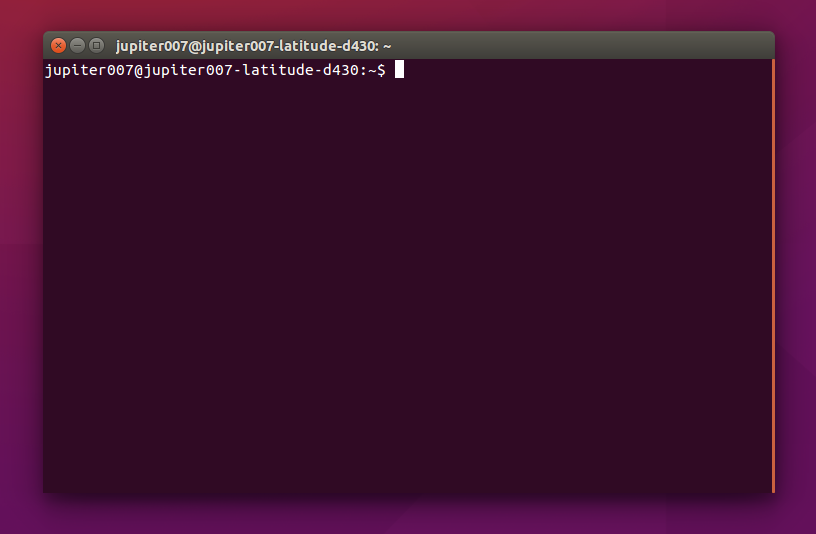
\includegraphics[width=8cm]{ressources/terminal.png}
\captionof{figure}{Un terminal sous Ubuntu}
\label{terminal}
\end{figure}

\emph{Windows} n'utilise pas les mêmes standards que les systèmes d'exploitation basés sur \emph{Unix}. Nous travaillerons sur un émulateur de terminal fonctionnant sur des systèmes \emph{Linux}. La page ci-après simule un terminal d'un système \emph{Linux}:
\begin{center}
\url{https://bellard.org/jslinux/vm.html?url=alpine-x86.cfg&mem=192}
\end{center}
Avant de commencer nous allons créer un compte utilisateur personnel en complétant le formulaire suivant:
\begin{center}
\url{https://vfsync.org/signup}
\end{center}
\begin{activite}
\begin{enumerate}
\item Créer un compte utilisateur.
\item Dans le terminale se connecter à son compte en tapant l'instruction ci-après dans \emph{l'invite de commande}.
\begin{lstlisting}
vflogin mon_identifiant
\end{lstlisting}
\item Remarquer que rien ne s'affiche quand le mot de passe est tapé. Pour quelle raison?
\end{enumerate}
\end{activite}
\section{Manipuler son espace}
\subsection{Arborescence}
Les systèmes basés sur les standards \emph{Unix} possèdent une arborescence de dossiers et fichiers identique (figure \ref{arbo}).
\begin{figure}[!h]
\centering
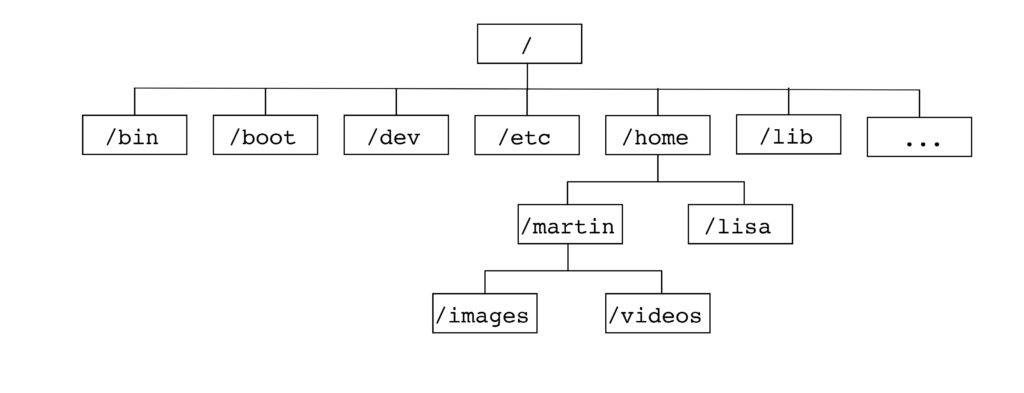
\includegraphics[width=15cm]{ressources/arborescence.jpg}
\captionof{figure}{Arborescence du système}
\label{arbo}
\end{figure}
\begin{itemize}
\item \guill{/} est le répertoire racine.
\item \guill{bin} contient les commandes de base.
\item \guill{etc} contient les fichiers de configuration système.
\item \guill{home} contient les répertoires personnels des utilisateurs.
\end{itemize}
\subsection{Se déplacer dans les dossiers}
L'invite de commande nous donne déjà des informations.
\begin{lstlisting}
localhost:~$
\end{lstlisting}
\begin{itemize}
\item \emph{localhost} indique la machine sur laquelle nous travaillons.
\item $\sim$ indique le répertoire où nous nous trouvons. Ce signe est particulier. C'est un raccourci qui pointe vers le dossier personnel de l'utilisateur.
\item \$ indique que l'utilisateur à la main et peut entrer une instruction.
\end{itemize}
\begin{activite}
\begin{enumerate}
\item Taper la commande \textbf{pwd}. Elle indique le dossier courant.
\item Taper l'instruction ci-après. La commande \textbf{cd} permet de naviguer dans les répertoires.
\begin{lstlisting}
cd /bin
\end{lstlisting}
\textbf{À retenir:} L'adresse est \emph{absolue} c'est à dire qu'elle démarre de la racine /
\item Dans quel dossier sommes-nous situé?
\item Se rendre dans le dossier \emph{home}.
\item Taper l'instruction ci-après (en remplaçant \emph{mon\_identifiant}).
\begin{lstlisting}
cd mon_identifiant
\end{lstlisting}
\textbf{À retenir:} L'adresse est \emph{relative} c'est à dire qu'elle démarre du répertoire courant. Nous la reconnaissons car elle ne commence pas par /
\item Dans quel dossier sommes-nous situé?\\
\textbf{À retenir:} L'instruction
\begin{lstlisting}
cd ..
\end{lstlisting}
permet de remonter d'un niveau de répertoire.
\end{enumerate}
\end{activite}
\subsection{Créer des dossiers}
\begin{activite}
\begin{enumerate}
\item Se placer dans le répertoire personnel.
\item Taper l'instruction ci-après. La commande \textbf{mkdir} crée un répertoire.
\begin{lstlisting}
mkdir images
\end{lstlisting}
\item Créer un répertoire \emph{devoir} dans le répertoire personnel.
\item Créer un répertoire \emph{photos\_vacances} dans le répertoire \emph{images}.
\end{enumerate}
\end{activite}
\subsection{Visualiser l'arborescence}
\begin{activite}
\begin{enumerate}
\item Taper l'instruction ci-après. La commande \textbf{ls} liste les répertoires et fichiers du répertoire donné.
\begin{lstlisting}
ls ~
\end{lstlisting}
Il est possible d'utiliser la commande \textbf{ls} seule. Elle renvoie alors la liste des répertoires et fichiers du répertoire courant.
\item Se placer dans le répertoire \emph{home}.
\item Taper \textbf{ls} puis les premières lettres du nom d'utilisateur. Appuyer sur la touche tabulation.\\
\textbf{À retenir:} La touche \emph{Tabulation} permet d'auto-compléter les noms de fichiers ou répertoires.
\item Taper l'instruction ci-après. Que fait-elle?
\begin{lstlisting}
tree
\end{lstlisting}
\end{enumerate}
\end{activite}
\subsection{Manipuler des fichiers}
Pour importer des fichiers dans cette simulation, il faut utiliser l'icône en bas de l'écran (figure \ref{up}).
\begin{figure}[!h]
\centering

\includegraphics[width=1cm]{ressources/upload-icon.png}
\captionof{figure}{Importer un fichier dans la simulation}
\label{up}
\end{figure}
\begin{activite}
\begin{enumerate}
\item Importer une image dans le répertoire personnel.
\item Taper l'instruction ci-après (en adaptant le nom de l'image). L'instruction \textbf{mv} déplace un fichier ou un répertoire. Le / à la fin de \emph{images} est important. Il indique que nous avons affaire à un répertoire.
\begin{lstlisting}
mv mon_image.jpg images/
\end{lstlisting}
\item Se rendre dans le dossier \emph{Images}.
\item Taper l'instruction ci-après (en adaptant le nom de l'image). L'instruction \textbf{cp} copie un fichier (ou un répertoire avec l'option -R).
\begin{lstlisting}
cp mon_image.jpg copie.jpg
\end{lstlisting}
\end{enumerate}
\end{activite}
\section{Les permissions}
Chaque fichier ou répertoire appartient à un utilisateur. Il peut y avoir plusieurs utilisateurs pour une même machine et certains documents peuvent avoir un caractère privé alors que d'autres sont utilisables par plusieurs personnes.
\begin{activite}
\begin{enumerate}
\item Se rendre dans le dossier \emph{images}.
\item Taper l'instruction ci-après.
\begin{lstlisting}
ls -l
\end{lstlisting}
\item Lire le cours \emph{openclassrooms} sur les droits d'accès:
\begin{center}
\url{https://tinyurl.com/yy9xmpa5}
\begin{commentprof}
\url{https://openclassrooms.com/fr/courses/43538-reprenez-le-controle-a-laide-de-linux/39044-les-utilisateurs-et-les-droits#/id/r-39043}
\end{commentprof}
\end{center}
\item Qui peut lire le fichier \emph{mon\_image.jpg}?
\item Donner à tout le monde \emph{le droit en lecture} de l'image.
\item Donner au groupe \emph{le droit en lecture et écriture} du dossier \emph{photos\_vacances}.
\end{enumerate}
\end{activite}
\end{Form}
\end{document}